% =====================================================================
% Semana 2 · S2.2 — Tolerancia del divisor (peor caso)
% Fundamentos de Sistemas Electrónicos Analógicos (Ingeniería Aeroespacial)
% Compilar: pdflatex semana_2_s22_tolerancia_divisor.tex  (2 pasadas)
% =====================================================================
\documentclass[aspectratio=169]{beamer}

\usepackage[utf8]{inputenc}
\usepackage[T1]{fontenc}
\usepackage{lmodern}
\usepackage[spanish,es-tabla]{babel}
\usepackage{amsmath,amssymb}
\usepackage{siunitx}
\usepackage{booktabs}
\usepackage{microtype}
\usepackage{circuitikz}

\definecolor{navy}{RGB}{23,54,93}
\definecolor{navysoft}{RGB}{72,101,140}
\definecolor{gold}{RGB}{179,142,62}
\definecolor{ink}{RGB}{44,51,58}
\definecolor{soft}{RGB}{244,241,234}

\usetheme{default}
\setbeamertemplate{navigation symbols}{}
\setbeamertemplate{footline}[frame number]
\setbeamercolor{structure}{fg=navy}
\setbeamercolor{frametitle}{fg=white,bg=navy}
\setbeamercolor{title}{fg=navy}
\setbeamercolor{subtitle}{fg=navysoft}
\setbeamercolor{itemize item}{fg=gold}
\setbeamercolor{itemize subitem}{fg=gold}
\setbeamercolor{block title}{fg=white,bg=navy}
\setbeamercolor{block body}{bg=soft}
\setbeamercolor{example text}{fg=navy}
\setbeamertemplate{itemize item}{\scriptsize\raise1.25pt\hbox{\donotcoloroutermaths$\bullet$}}
\setbeamertemplate{itemize subitem}{\scriptsize\raise1.25pt\hbox{\donotcoloroutermaths$\circ$}}
\setbeamerfont{frametitle}{size=\large,series=\bfseries}

\title[S2.2 · Tolerancia del divisor]{Tolerancia del divisor y análisis de peor caso}
\subtitle{S2.2 — Simulaciones y laboratorio de la Semana 2}
\institute{Licenciatura en Ingeniería Aeroespacial\\ UNAM · ENES Unidad Juriquilla}
\author{M. en C. José de Jesús Santana Ramírez}
\date{Semestre 2027-1}

\begin{document}

% ---------------------------------------------------------------------
\begin{frame}[plain]
  \titlepage
\end{frame}

% ---------------------------------------------------------------------
\begin{frame}{Objetivos de la sesión}
  \begin{itemize}
    \item Interpretar la \textbf{tolerancia} de un resistor ($\pm 1\,\text{\%}$, serie E96) y su efecto en la salida.
    \item Evaluar las \textbf{cuatro combinaciones extremas} de dos resistores de $1\,\text{\%}$ (peor caso).
    \item Comparar el \textbf{rango de salida} con el valor nominal.
    \item Distinguir \textbf{error de razón} de \textbf{error de valor absoluto}.
  \end{itemize}
  \pause
  \begin{block}{Pregunta}
    Si ambos resistores de un divisor cambian de valor por la temperatura, ¿la salida cambia?
  \end{block}
\end{frame}

% ---------------------------------------------------------------------
\begin{frame}{Teoría 1 · Tolerancia y análisis de peor caso}
  La tolerancia es el desvío máximo del valor real respecto del nominal. Un
  resistor de $1\,\text{k}\Omega$ con $\pm 1\,\text{\%}$ puede medir entre
  $\SI{990}{\ohm}$ y $\SI{1010}{\ohm}$.
  \pause
  \begin{itemize}
    \item En un divisor, la salida depende de la \textbf{razón} $R_2/(R_1+R_2)$, no del valor absoluto.
    \item \textbf{Peor caso:} cuando las tolerancias se combinan en la dirección más desfavorable.
    \item Se evalúan las $2^2 = 4$ combinaciones de $\pm 1\,\text{\%}$ de $R_1$ y $R_2$.
  \end{itemize}
\end{frame}

% ---------------------------------------------------------------------
\begin{frame}{Teoría 2 · Error de razón contra error de valor absoluto}
  \begin{itemize}
    \item \textbf{Error de valor absoluto:} ambos resistores cambian en la misma proporción.
      Ej.: $R_1 = 1010\,\Omega$, $R_2 = 1010\,\Omega$ $\Rightarrow$ la razón sigue siendo $0.5$.
    \item \textbf{Error de razón:} cambian en proporciones distintas.
      Ej.: $R_1 = 990\,\Omega$, $R_2 = 1010\,\Omega$ $\Rightarrow$ la razón se desplaza.
  \end{itemize}
  \[
    V_{out} = V_{in}\cdot\frac{R_2}{R_1+R_2}
    \qquad
    \text{error}_{\%} = 100\cdot\frac{V_{out}-V_{out}^{nom}}{V_{out}^{nom}}
  \]
  \pause
  \begin{block}{Idea clave}
    Un divisor es un \textbf{transductor de razón}: los cambios \emph{comunes} (mismo signo)
    se cancelan; los cambios \emph{diferenciales} (signos opuestos) generan error.
  \end{block}
\end{frame}

% ---------------------------------------------------------------------
\begin{frame}{Ejercicio · Enunciado}
  \begin{block}{Divisor 1:1 con resistores de $\pm 1\,\text{\%}$}
    \centering
    $V_{in} = \SI{5}{\volt}$, \quad $R_1 = R_2 = 1\,\text{k}\Omega\ (\pm 1\,\text{\%})$, \quad salida nominal $\SI{2.5}{\volt}$.
  \end{block}
  \begin{center}
    \resizebox{0.62\linewidth}{!}{%
    \begin{circuitikz}[american voltages, scale=0.95]
      \draw (0,3) to[V, l={$V_{in}=5\,\mathrm{V}$}, i=$I$] (0,0);
      \draw (0,3) -- (1.4,3) to[R, l={$R_1$}] (4.4,3);
      \draw (4.4,3) -- (5.3,3) to[R, l={$R_2$}] (5.3,0);
      \draw (5.3,0) -- (0,0);
    \node[ground] at (0,0) {};
    \end{circuitikz}}
  \end{center}
  \textbf{Determinar:} la salida para las 4 combinaciones de $\pm 1\,\text{\%}$ y el rango total de error.
\end{frame}

% ---------------------------------------------------------------------
\begin{frame}{Desarrollo · Cuatro combinaciones extremas}
  \begin{table}
    \small
    \begin{tabular}{cccccc}
      \toprule
      Caso & $T_1$ & $T_2$ & $R_1$ & $R_2$ & $V_{out}$ (error) \\
      \midrule
      0 & $-1\,\text{\%}$ & $-1\,\text{\%}$ & $\SI{990}{\ohm}$  & $\SI{990}{\ohm}$  & $\SI{2.500}{\volt}$ \ (0\,\text{\%}) \\
      1 & $-1\,\text{\%}$ & $+1\,\text{\%}$ & $\SI{990}{\ohm}$  & $\SI{1010}{\ohm}$ & $\SI{2.525}{\volt}$ \ ($+1.0\,\text{\%}$) \\
      2 & $+1\,\text{\%}$ & $-1\,\text{\%}$ & $\SI{1010}{\ohm}$ & $\SI{990}{\ohm}$  & $\SI{2.475}{\volt}$ \ ($-1.0\,\text{\%}$) \\
      3 & $+1\,\text{\%}$ & $+1\,\text{\%}$ & $\SI{1010}{\ohm}$ & $\SI{1010}{\ohm}$ & $\SI{2.500}{\volt}$ \ (0\,\text{\%}) \\
      \bottomrule
    \end{tabular}
  \end{table}
  \pause
  \begin{itemize}
    \item Los casos 0 y 3 (mismo signo) dan error nulo: la razón se conserva.
    \item Los casos 1 y 2 (signos opuestos) dan el error máximo: $\pm 1\,\text{\%}$.
  \end{itemize}
\end{frame}

% ---------------------------------------------------------------------
\begin{frame}{Desarrollo · Verificación y lectura}
  \[
    \text{caso 1:}\quad V_{out} = 5\cdot\frac{1010}{990+1010} = \SI{2.525}{\volt}
    \qquad
    \text{caso 2:}\quad V_{out} = 5\cdot\frac{990}{1010+990} = \SI{2.475}{\volt}
  \]
  \pause
  \begin{block}{Lectura de diseño}
    El rango de salida es $\SI{2.475}{\volt}$ a $\SI{2.525}{\volt}$ ($\pm 1\,\text{\%}$).
    \begin{itemize}
      \item Si la etapa siguiente (ADC, amplificador) requiere $2.5\,\text{V}\pm 0.5\,\text{\%}$, este
        divisor $\pm 1\,\text{\%}$ \textbf{no basta}: se usan resistores de $0.1\,\text{\%}$ o se calibra.
      \item El error de \emph{valor absoluto} (ambos iguales) no afecta la razón, pero sí la
        corriente y la potencia consumidas.
    \end{itemize}
  \end{block}
\end{frame}

% ---------------------------------------------------------------------
\begin{frame}[fragile]{Verificación en LTspice}
  Abrir \texttt{semana2\_02\_divisor\_tolerancia.cir} (barrido de caso $0$ a $3$) y consultar el Error Log:

  \begin{verbatim}
.meas op VOUT FIND V(vout)
.meas op ERROR_PCT PARAM 100*(V(vout)-2.5)/2.5
  \end{verbatim}

  \textbf{Criterio de éxito:} casos 0/3 $\rightarrow$ error $\approx 0$; casos 1/2 $\rightarrow$
  error $\approx \pm 1\,\text{\%}$.
\end{frame}

% ---------------------------------------------------------------------
  % ---------------------------------------------------------------------
  \begin{frame}{Resultado de la simulación}
    \begin{center}
      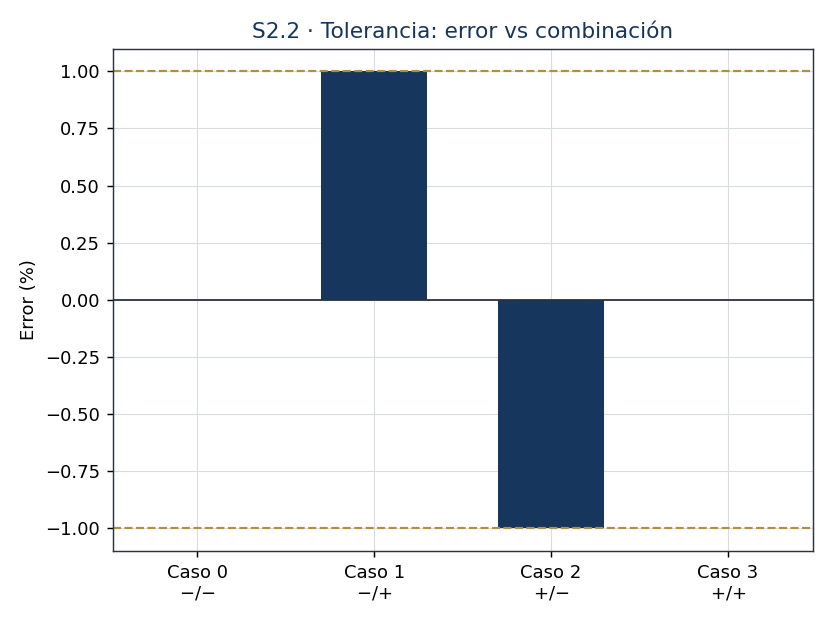
\includegraphics[width=0.78\textwidth]{figs/s22_tolerancia.png}
    \end{center}
    \begin{itemize}
      \item Solo los casos de signos opuestos generan error ($\pm 1\%$).
    \end{itemize}
  \end{frame}

  % ---------------------------------------------------------------------
  \begin{frame}{Errores comunes}
  \begin{table}
    \small
    \begin{tabular}{p{0.34\textwidth}p{0.30\textwidth}p{0.30\textwidth}}
      \toprule
      Error & Consecuencia & Corrección \\
      \midrule
      Sumar tolerancias en valor absoluto & Sobreestimar el error & Evaluar ambos signos (peor caso) \\
      Asumir que cambiar $R_1$ y $R_2$ igual no afecta & Perder el rango exacto & La razón se conserva, pero no la corriente \\
      Olvidar el rango de temperatura & Deriva en vuelo & Modelar TCR y extremos ambientales \\
      Ignorar que el ADC también tiene error & Presupuesto incompleto & Sumar errores (WCCA, RSS) \\
      \bottomrule
    \end{tabular}
  \end{table}
\end{frame}

% ---------------------------------------------------------------------
\begin{frame}{Lectura aeroespacial}
  \begin{itemize}
    \item \textbf{Divisores de referencia:} en la referencia de un ADC se requieren resistores de
      $0.1\,\text{\%}$ y bajo TCR; el $\pm 1\,\text{\%}$ de un divisor de potencia no es aceptable.
    \item \textbf{Deriva térmica:} ambos resistores suelen ser del mismo material y lotes; su
      deriva \emph{común} se cancela en la razón (bueno), pero el desajuste entre ellos (\emph{tracking})
      genera error.
    \item \textbf{WCCA:} el análisis de peor caso (tolerancias + deriva + envejecimiento) se hace con
      las combinaciones extremas para garantizar que la salida quede dentro del rango del ADC.
    \item \textbf{Calibración en banco:} si la tolerancia individual es desconocida, se mide el valor
      real y se calcula el error; esto es habitual en el acondicionamiento de galgas.
  \end{itemize}
\end{frame}

% ---------------------------------------------------------------------
\begin{frame}{Preguntas de verificación}
  \begin{enumerate}
    \item ¿Por qué los casos 0 y 3 (mismo signo) dan error nulo en un divisor 1:1?
    \item ¿Cuál es el peor caso: tolerancias del mismo signo o de signos opuestos?
      \uncover<2->{\emph{(Signos opuestos: desplazan la razón.)}}
    \item ¿Qué cambia si el divisor no es 1:1 (p. ej. $R_1 = 3\,\text{k}$, $R_2 = 1\,\text{k}$) con $\pm 1\,\text{\%}$?
    \item Si se necesitan $\pm 0.5\,\text{\%}$: ¿qué opciones tiene el diseñador?
      \uncover<3->{\emph{(Resistores de menor tolerancia, calibración, o red de ajuste.)}}
    \item ¿El error de valor absoluto importa si la señal va a un ADC de razón (ratiometric)?
  \end{enumerate}
\end{frame}


\end{document}
